\documentclass[a4paper,english,12pt]{article}
\usepackage{%
	amsfonts,%
	amsmath,%	
	amssymb,%
	amsthm,%
	algorithm,%
	babel,%
	bbm,%
	etex,%
	%biblatex,%
	caption,%
	centernot,%
	color,%
	dsfont,%
	enumerate,%
	epsfig,%
	epstopdf,%
	geometry,%
	graphicx,%
	hyperref,%
	latexsym,%
	mathtools,%
	multicol,%
	pgf,%
	pgfplots,%
	pgfplotstable,%
	pgfpages,%
	proof,%
	psfrag,%
	subfigure,%	
	tikz,%
	ulem,%
	url%
}	
\usepackage[noend]{algpseudocode}
\usepackage[mathscr]{eucal}
\usepgflibrary{shapes}
\usetikzlibrary{%
  	arrows,%
	backgrounds,%
	chains,%
	decorations.pathmorphing,% /pgf/decoration/random steps | erste Graphik
	decorations.text,%
	matrix,%
  	positioning,% wg. " of "
  	fit,%
	patterns,%
  	petri,%
	plotmarks,%
  	scopes,%
	shadows,%
  	shapes.misc,% wg. rounded rectangle
  	shapes.arrows,%
	shapes.callouts,%
  	shapes%
}

\theoremstyle{plain}
\newtheorem{thm}{Theorem}[section]
\newtheorem{lem}[thm]{Lemma}
\newtheorem{prop}[thm]{Proposition}
\newtheorem{cor}[thm]{Corollary}

\theoremstyle{definition}
\newtheorem{defn}[thm]{Definition}
\newtheorem{conj}[thm]{Conjecture}
\newtheorem{exmp}[thm]{Example}
\newtheorem{assum}[thm]{Assumptions}
\newtheorem{axiom}[thm]{Axiom}

\theoremstyle{remark}
\newtheorem{rem}{Remark}
\newtheorem{note}{Note}
\newtheorem{fact}{Fact}

\newcommand{\norm}[1]{\left\lVert#1\right\rVert}
\newcommand{\indep}{\!\perp\!\!\!\perp}
\DeclarePairedDelimiter\abs{\lvert}{\rvert}%
\newcommand\numberthis{\addtocounter{equation}{1}\tag{\theequation}}
\newcommand{\tr}{\operatorname{tr}}
\newcommand{\R}{\mathbb{R}}
\newcommand{\N}{\mathbb{N}}
\newcommand{\E}{\mathbb{E}}
\newcommand{\Z}{\mathbb{Z}}
\newcommand{\B}{\mathscr{B}}
\newcommand{\C}{\mathcal{C}}
\newcommand{\T}{\mathscr{T}}
\newcommand{\F}{\mathcal{F}}
\newcommand{\G}{\mathcal{G}}
%\newcommand{\ba}{\begin{align*}}
%\newcommand{\ea}{\end{align*}}
\DeclareMathOperator*{\argmax}{arg\,max}
\renewcommand{\qedsymbol}{$\blacksquare$}
\makeatletter
\def\BState{\State\hskip-\ALG@thistlm}
\makeatother

\makeatletter
\def\th@plain{%
  \thm@notefont{}% same as heading font
  \itshape % body font
}
\def\th@definition{%
  \thm@notefont{}% same as heading font
  \normalfont % body font
}
\makeatother
\date{}

%opening
\title{Lecture 6: Composite Hypothesis Testing and Properties of a Random Sample}
\date{28 Jan 2016}
\author{}

\begin{document}
\maketitle
In the previous lecture, the Bayesian formulation for a composite hypothesis testing problem has been shown. In this lecture, some examples of composite hypothesis testing problems are considered. Further, the notion of a random sample has been defined and some of its properties have been listed and proved.
\section{Examples of a composite hypothesis testing problem}
Let us consider the following example of a composite hypothesis testing problem.
\begin{exmp}
Testing on the radius of a point on the plane:
\par Suppose that $\Gamma = {\mathbb{R}}^2$ , i.e. $Y \in \Gamma$, $Y = (Y_1,Y_2).$
\begin{align*}
Y &= X + n,\\
\mbox{where, }
n &\sim \mathcal{N}(0,\sigma^2I_2),\nonumber\\
X &\in \{0,(A\cos\psi,A\sin\psi)\}.\nonumber
\end{align*}
$A > 0$, a constant, $\psi \sim$ unif($[0,2\pi)$) and $n_1$ and $n_2$ are independent of one another and of $\psi$. The null hypothesis and the alternate hypothesis are given by,
\begin{align*}
\mathcal{H}_0 &: Y \sim \mathcal{N}(0,\sigma^2I_2).\\
\mathcal{H}_1 &: Y \sim \mathcal{N}((A\cos\psi,A\sin\psi),\sigma^2I_2).
\end{align*}	
The observation is a noisy measurement of the coordinates of a point in the plane that is either at the origin or is uniform-randomly distributed on a circle of radius $A$.
\begin{figure}
\centering
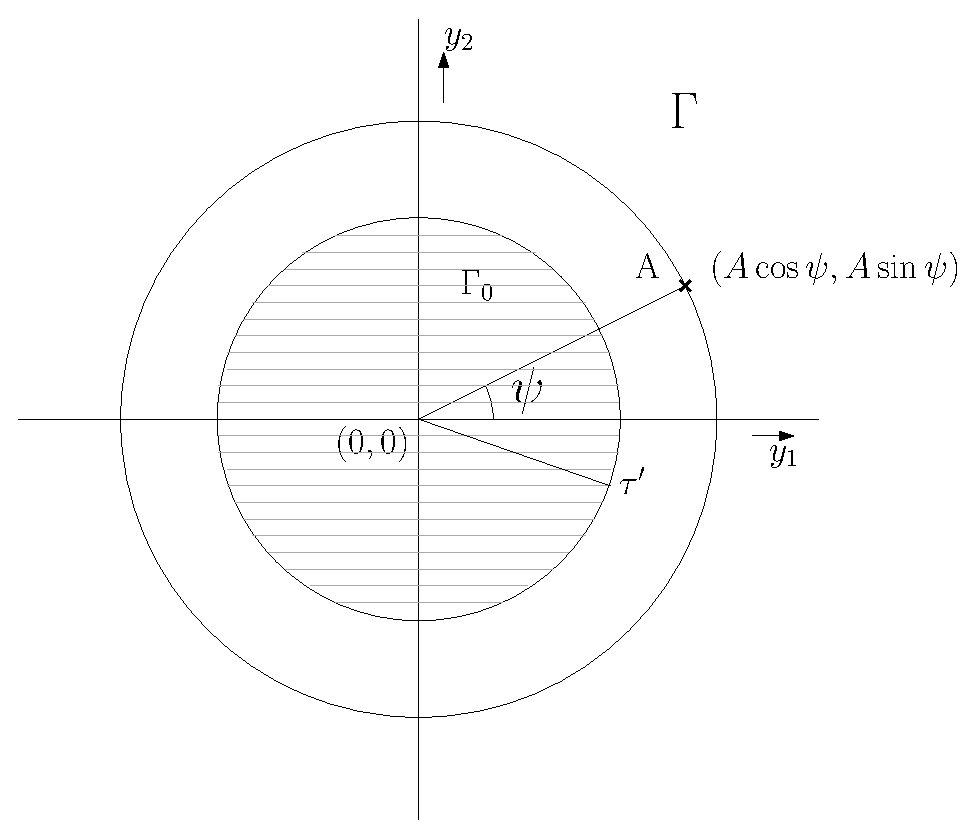
\includegraphics[scale=0.4]{Figures/decisionRegions.eps}
\caption{Decision regions for example 1.1($\Gamma_1 = \Gamma_0^c$).}
\label{fig: example 1.1}
\end{figure}	
So, we have partitions of parametric family of different distributions. For each $\psi$, we get different distributions.
\par Let the parameter be $\Theta = (\Theta_1,\Theta_2)$, with $\Theta_1 \in \{0,A\}$ and $\Theta_2 \in [0,2\pi)$. Thus the parameter set is $\Lambda = \{0,A\}\times [0,2\pi),$ with $\Lambda_0 = \{\theta \in \Lambda : \theta_1 = 0\}$ and $\Lambda_1 = \{\theta \in \Lambda : \theta_1 = A\}$. Let $\psi$ be a random variable that takes the value $\theta_2$. The conditional distribution of $Y$ given $\Theta = \theta$ is given by,
\begin{eqnarray}
Y|(\Theta=\theta) &\sim& \mathcal{N} ((\theta_1\cos\theta_2,\theta_1\sin\theta_2), \sigma^2I_2).\\
P_\theta(y) &=& \int_{-\infty}^{y_1}\int_{-\infty}^{y_2}\dfrac{1}{2\pi\sigma^2}\exp\Big[\dfrac{-q(u,\theta)}{2\sigma^2}\Big]du, ~~ y \in {\mathbb{R}}^2\\
\mbox{where,}\nonumber\\
q(y,\theta) &\triangleq& (y_1-\theta_1\cos\theta_2)^2 + (y_2-\theta_1\sin\theta_2)^2.
\end{eqnarray}	
The likelihood ratio calculation is as follows,
\begin{eqnarray}
p(y|\Theta \in \Lambda_0) &=& p_\theta(y)|_{\theta_1 = 0},\\
&=& \dfrac{1}{2\pi\sigma^2}\exp\big[-\dfrac{(y_1^2 + y_2^2)}{2\sigma^2}\big],\\
\mbox{and,}\nonumber\\
p(y|\Theta \in \Lambda_1)&=& \frac{1}{2\pi}\int_{0}^{2\pi}p_\theta(y)|_{\theta_1 = A}d\theta_2,\\
&=& \dfrac{1}{4\pi^2\sigma^2}\int_{0}^{2\pi}\exp\big[\frac{-q(y,\theta)|_{\theta_1 = A}}{2\sigma^2}\big]d\theta_2.
\end{eqnarray} 	
The likelihood ratio is thus given by,
\begin{equation}
L(y) = \frac{dP_1(y| \theta \in \Lambda_1)}{dP_0(y| \theta \in \Lambda_0)}
\end{equation}
Assume $c(i,\theta)$ is constant over $\theta \in \Lambda_1,~\theta \in \Lambda_0$.
\begin{eqnarray}
\frac{d}{dy}P_\Theta(y | \Theta \in \Lambda_1) &=& \mathbb{E}\big[P_\Theta(y | \Theta \in \Lambda_1), \Theta_2]. \\
&=& \dfrac{1}{2\pi}\int_{0}^{2\pi}\exp\Big[\dfrac{-q(y,\theta)}{2\sigma^2}\Big]d\theta_2 ~ \forall ~ \theta \in \Lambda.
\end{eqnarray}	
Rewriting the likelihood ratio $L(y)$ as,
\begin{equation*}
L(y) = \frac{1}{2\pi}\int_{0}^{2\pi}\dfrac{\exp\Big[\frac{-1}{2{\sigma}^2}\Big({y_1}^2 + A^2{\cos\theta_2}-2y_1A\cos\theta_2\Big)-\frac{1}{2{\sigma}^2}\Big({y_2}^2 + A^2{\sin\theta_2}-2y_2A\sin\theta_2\Big)\Big]}{\exp\Big(-\dfrac{({y_1}^2 + {y_2}^2)}{2{\sigma}^2}\Big)}d\theta_2.
\end{equation*}
\begin{eqnarray}
L(y) &=& \frac{1}{2\pi}\int_{0}^{2\pi}\exp\Big[-\frac{A^2}{2{\sigma}^2}+\frac{A}{{\sigma}^2}(y_1\cos\theta_2 + y_2\sin\theta_2)\Big]d\theta_2, \nonumber \\
&=&\dfrac{\exp\big(-\frac{A^2}{2{\sigma}^2}\big)}{2\pi}\int_{0}^{2\pi}\exp\Big[\frac{A}{{\sigma}^2}(y_1\cos\theta_2 + y_2\sin\theta_2)\Big]d\theta_2.
\end{eqnarray}
Using the following transformation of variables to make simplifications in the integral,
\begin{eqnarray}
r^2 &=& {y_1}^2 + {y_2}^2,~\mbox{and}~\tan\phi =\frac{y_2}{y_1},\\\nonumber
L(r) &=& \dfrac{\exp\big(-\frac{A^2}{2\sigma^2}\big)}{2\pi}\int_{0}^{2\pi}\exp\big(\frac{A}{\sigma^2}r\cos(\theta_2 - \phi)\big)d\theta_2,\\
&=& \exp\big(-\frac{A^2}{2\sigma^2}\big)I_0\big(\frac{Ar}{\sigma^2}\big).
\end{eqnarray}
where $I_0(.)$ is the "zeroth order Bessel function of the first kind".
\begin{note} 
Notice that $L(y)$ is independent of $\phi$.
\end{note}
\begin{note}
$I_0$ is monotone increasing in its argument.
\end{note}
Let us denote the threshold by $\tau$. Since $I_0$ is a monotonic function, it can be inverted to find $r$.
\begin{eqnarray}
\nonumber
L(r) &=& \tau.\\\nonumber
r &=& L^{-1}(\tau) = \tau'.\\
\tau' &=& \frac{\sigma^2}{A}I_0^{-1}\Big(\exp\big(\frac{A^2}{2\sigma^2}\big)\Big).
\end{eqnarray}
The decision rule is,
\begin{eqnarray}
\tilde{\delta}(y) &=&
\begin{cases}
1, &\mbox{if}~ r > \tau'.\\
\gamma, &\mbox{if}~ r = \tau'.\\
0, &\mbox{if}~ r < \tau'.
\end{cases}
\end{eqnarray}
\end{exmp}
We have completely characterized decision rule for Bayesian framework. But we know that similar decision rules will hold for minimax. For composite hypothesis testing problems in which the prior distributions of the parameters are unknown, the definition of optimality requires a generalization of the Neyman-Pearson criterion of the simple hypothesis testing problem.
\par Recall, for a randomized decision rule $\tilde{\delta}$ we want to maximize probability of detection such that probability of false alarm is bounded by "significance level" $\alpha$.
\begin{eqnarray}
P_F(\tilde{\delta}; \theta) &=& \mathbb{E}_\theta\big(\tilde{\delta}(Y)\big), ~ \theta \in \Lambda_0.\\
P_D(\tilde{\delta}; \theta) &=& \mathbb{E}_\theta\big(\tilde{\delta}(Y)\big), ~ \theta \in \Lambda_1.
\end{eqnarray}	
This is well defined if there is a unique $\theta \in \Lambda_0$ and a unique $\theta \in \Lambda_1$. But the problem is that there are many $\theta$'s in $\Lambda_0$ and $\Lambda_1$.
\begin{defn}
A Uniformly Most Powerful (UMP) test is a decision rule that maximizes the probability of detection $\forall \theta \in \Lambda_1$, such that the probability of false alarm $\forall \theta \in \Lambda_0$ is below the significance level $\alpha$.
\begin{eqnarray*}
\max_{\tilde{\delta}}P_D(\tilde{\delta}; \theta), ~ \forall \theta \in \Lambda_1.\\
\mbox{s.t.  } P_F(\tilde{\delta}; \theta) \leq \alpha, ~ \forall \theta \in \Lambda_0.
\end{eqnarray*}	
\end{defn}
Although the UMP tests are desirable, they exist only in certain cases. To demonstrate this, let us consider the following example.
\begin{exmp} 
Consider a case where the null hypothesis is simple, i.e., $\Lambda_0 = \{\theta_0\}$, and the alternate hypothesis $\Lambda_1$ is composite. For each $\theta \in \Lambda_1$, we can find the rejection region.
\begin{eqnarray}
\Gamma_\theta &=& \{y \in \Gamma: L(y) > \tau\}.\\
\mbox{where  } L(y) &=& \dfrac{dP_{\theta_1}(y)}{dP_{\theta_0}},	
\end{eqnarray}		
is the likelihood ratio and $\tau$ is the threshold chosen(with possibly randomization) to give significance level $\alpha$. By the N-P lemma, we know that this test is unique, i.e., for $\theta_1, \theta_2 \in \Lambda_1$, such that $\theta_1 \neq \theta_2 $, the test with critical region $\Gamma_{\theta_1}$ will have smaller power in testing $\mathcal{H}_0: Y \sim P_{\theta_0}$ versus $\mathcal{H}_1: Y \sim P_{\theta_2}$ and vice versa unless the two critical regions are identical.	
\begin{equation*}
P_{\theta_{2}}(\Gamma_{\theta_1}) \leq P_{\theta_{2}}(\Gamma_{\theta_2}).
\end{equation*}
with equality iff $\Gamma_{\theta_1} = \Gamma_{\theta_2}$.
\begin{cor}
{A UMP test exists for simple $\mathcal{H}_0$ versus composite $\mathcal{H}_1$ iff $\Gamma_\theta$ is identical $\forall \theta \in \Gamma_1$.}	
\end{cor}
\end{exmp}

\begin{exmp}{UMP testing of location:}
\par Consider the parametric family of distributions $\{P_\theta;\theta \in \Lambda\}$, where, 
\begin{equation}
\{P_\theta= \mathcal{N}(\theta,\sigma^2),~\theta \in \Lambda\}, ~ \Lambda \subseteq \mathbb{R},
\end{equation}
and, suppose that we have the hypotheses,
\begin{eqnarray}
\mathcal{H}_0 : \theta = \mu_0,\\
\mathcal{H}_1 : \theta > \mu_0.	
\end{eqnarray}
That is, $\Lambda_0 = \{\mu_0\}$ and $\Lambda_1 = (\mu_0,\infty)$. The most powerful $\alpha$-level test $\mathcal{H}_0$ versus $\mathcal{H}_1 : Y \sim \mathcal{N}(\theta,\sigma^2)$ has critical region:
\begin{equation*}
\Gamma_\theta = \{y \in \Gamma: y > \sigma \Phi^{-1}(1 - \alpha) + \mu_0 \}, ~ \forall ~ \theta \in \Lambda_1.
\end{equation*}
The UMP test, denoted by $\tilde{\delta}$ is:
\begin{equation*}
\tilde{\delta} = \mathbbm{1}_{\{y \in \Gamma_\theta\}}.
\end{equation*}
\begin{rem}
Randomization is not required since the continuous random variables are being considered.	
\end{rem}		
\begin{equation*}
P_D(\tilde{\delta}; \theta) = 1 - \Phi\Big(\Phi^{-1}(1 - \alpha) - \dfrac{(\theta - \mu_0)}{\sigma}\Big).
\end{equation*}
\begin{note}
	$\Gamma_\theta$ does not depend on $\theta$.	
\end{note}	
\begin{note}
	In this case we found a UMP; but this is rather rare.	
\end{note}	
\end{exmp}		 
\begin{exmp}{Testing of location with different hypotheses pair:}
\par The setup is as in the previous example, except a different $\mathcal{H}_1$.
\begin{align*}
\mathcal{H}_0 &: \theta = \mu_0  \text{   (as before),}\\
\mathcal{H}_1 &: \theta \neq \mu_0.
\end{align*}
That is, $\Lambda_0 = \{\mu_0\}$ and $\Lambda_1 = (-\infty, \mu_0) \bigcup (\mu_0, \infty)$.\\
For $\theta > \mu_0$, the most powerful test is
\begin{equation}
\tilde{\delta_1}(y) = \mathbbm{1}_{\{y \in \Gamma_\theta\}},
\end{equation}
and the critical region is
\begin{equation}
\Gamma_\theta^1 = \{y \in \Gamma: y > \sigma\Phi^{-1}(1 - \alpha) + \mu_0\},
\end{equation}
as in the previous example.
\par Now, we consider the case when $\theta < \mu_0$. The critical region of the most powerful $\alpha$-level test becomes:
\begin{equation}
\Gamma_\theta^2 = \{y \in \Gamma: y < \sigma\Phi^{-1}(\alpha) + \mu_0\}.
\end{equation}
The most powerful test being,
\begin{equation}
\tilde{\delta_2}(y) = \mathbbm{1}_{\{y \in \Gamma_\theta^2\}},
\end{equation}
resulting in the power of test,
\begin{equation}
P_D(\tilde{\delta_2}; \theta) = \Phi\Big(\Phi^{-1}(\alpha) - \dfrac{(\theta - \mu_0)}{\sigma}\Big).
\end{equation}
\begin{figure}
\centering
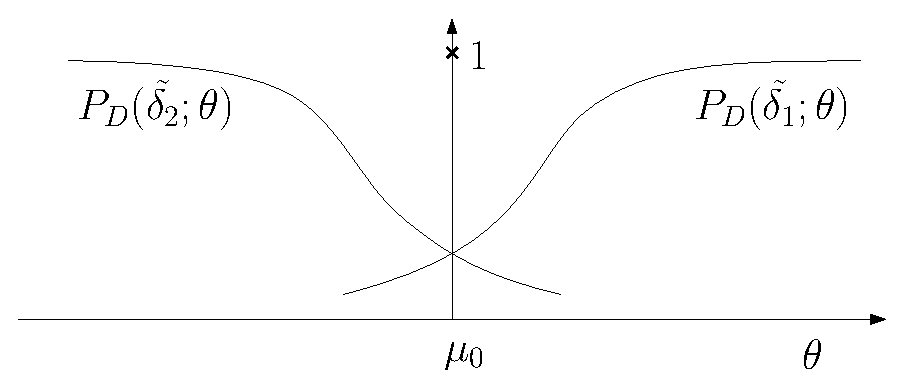
\includegraphics[scale=0.6]{Figures/PD.eps}
\caption{Power curves for test of $\theta = \mu_0$ versus $\theta > \mu_0$ and $\theta = \mu_0$ versus $\theta < \mu_0$, for location testing with Gaussian error.}
\label{fig: example 1.5 and 1.6}
\end{figure}
\end{exmp}
\begin{rem}
Although the critical region is independent of $\theta$, it is different from the critical region for the case of $\theta > \mu_0$. Thus, no UMP exists. So we come up with some other criteria.
\end{rem}
\begin{rem}
Although the UMP is optimal in some sense, it is rare.
\end{rem}
\begin{rem}
The UMP is thus too strong a criterion for many situations.
\end{rem}
\section*{Other criteria}
As observed earlier, the UMP criterion is very strong to be satisfied. Hence by applying some reasonable constraints, we consider a few other criteria.
\begin{enumerate}
\item \textbf{Unbiasedness}
\begin{defn}{A test is said to satisfy the condition of unbiasedness if,
\begin{eqnarray*} 
P_D(\tilde{ \delta};\theta)&\geq&\alpha,  ~ \forall  \theta \in  \Lambda_1, \\
\mbox{in addition to}\\
P_F(\tilde{\delta};\theta) &\leq& \alpha,  ~ \forall  \theta \in  \Lambda_0.
\end{eqnarray*}
}
\end{defn}	
This requirement would eliminate both $\tilde{\delta}_1$ and $\tilde{\delta}_2$ in the previous example.  
\begin{exmp} Consider an example where the parameter set is given by $\Lambda = [\theta_0,\infty).$ Let $\Lambda_0 = \{\theta_0\}, ~ \Lambda_1 = (\theta_0, \infty)$. The null hypothesis and the alternate hypothesis are given by:
\begin{eqnarray}
\mathcal{H}_0 : \theta = \theta_0, \\ 
\mathcal{H}_1 : \theta > \theta_0.
\end{eqnarray}
Such a case arises in signal detection where the amplitude of the signal is represented by $\theta$.
\par The only case where confusion arises is when the received amplitude is close to $\theta_0$. Consider a decision rule $\tilde{\delta}$. Under certain regularity conditions, by the application of Taylor's series expansion about $\theta_0$, we obtain,
\begin{eqnarray}
P_D(\tilde{ \delta};\theta) &=& P_D(\tilde{ \delta};\theta_0) + (\theta - \theta_0) P_{D}'(\tilde{ \delta};\theta_0) + O((\theta - \theta_0)^2). \nonumber \\
&=&P_F(\tilde{ \delta}) + (\theta - \theta_0) P_{D}'(\tilde{ \delta};\theta_0) + O((\theta - \theta_0)^2). \nonumber \\
&\approxeq& \alpha + (\theta - \theta_0) P_{D}'(\tilde{ \delta};\theta_0).
\end{eqnarray} 
\end{exmp}
\item \textbf{$\alpha$-level "locally most powerful test" (LMP)}
\par A test that maximizes $P_{D}'(\tilde{\delta};\theta_0)$ subject to false alarm constraint $P_F(\tilde{\delta}) \leq \alpha$ is called an $\alpha$-level locally most powerful test (LMP).
\begin{eqnarray}
\max\limits_{\tilde{\delta}} P_{D}'(\tilde{\delta};\theta_0), \\\nonumber 
\mbox{subject to }P_F(\tilde{\delta}) \leq \alpha.
\end{eqnarray}
Consider,
\begin{align}
P_D(\tilde{ \delta};\theta) &= \mathbb{E}_\theta \{\tilde{ \delta}(Y)\}, \nonumber \\
&= \int_{y \in \Gamma}  \tilde{\delta}(y) dP_\theta(y). \nonumber \\
P_{D}'(\tilde{ \delta};\theta_0) &=  \int\limits_{y \in \Gamma}  \tilde{\delta}(y) d\Bigg[\frac{\partial}{\partial \theta}P_\theta(y)\Bigg]_{\theta = \theta_0},~\mbox{and} \nonumber \\
\tilde{\delta}_{LO}(y) &= 
\begin{cases} 
1, &\mbox{if}~ [\frac{\partial}{\partial \theta}L(y) ] \mid_{\theta = \theta_0} > \eta. \\
\gamma, &\mbox{if}~ [\frac{\partial}{\partial \theta}L(y)] \mid_{\theta = \theta_0} = \eta. \\
0, &\mbox{if}~ [\frac{\partial}{\partial \theta}L(y) ] \mid_{\theta = \theta_0} < \eta.
\end{cases}
\end{align}
We are mostly interested in the case when $\Lambda_0 = \{\theta_0\}$ and $\Lambda_1$ is composite, where $\eta$ and $\gamma$ are chosen such that, 
\begin{equation*}
P_F(\tilde{\delta}_{LO}) = \alpha.
\end{equation*}
\item \textbf{Maximum Likelihood Test}
\par A test that is applicable for composite hypothesis testing problems is based on comparaing the likelihood ratio $ L(y)$ to a threshold $\tau$. The likelihood ratio is given by,
\begin{equation}
L(y)=\dfrac{\max\limits_{\theta \in \Lambda_1} ~ dP_\theta(y)}{\max\limits_{\theta \in \Lambda_0} ~ dP_\theta(y)}. 
\end{equation}
So, we have three ways to deal with the composite hypothesis test.
\end{enumerate}
\section{Properties of a random sample}
In this section, we define a random sample and its statistics. Also, some properties of the random sample are listed and proved.
\begin{defn}
The collection of random variables $X_1, X_2, .... X_n$ is called a "random sample of size $n$ from the population $p(X)$", if they are independent and identically distributed with common distribution $p$.
The joint pdf of $X_1, X_2, .... X_n$ is given by 
\begin{equation}
p(x_1,x_2,...x_n) = p(x_1) p(x_2)...p(x_n) = \prod\limits_{i=1}^{n} p_X(x_i).
\end{equation} 
\end{defn}
\begin{defn}
Let $X_1, X_2, .... X_n$ be a random sample of size $n$ from the population $p(X)$ and let $T$ be a real/vector valued function whose domain includes the sample space of $X_1, X_2, .... X_n$. Then the random variable/vector $Y = T(X_1, X_2, .... X_n)$ is called a "statistic". The probability distribution of the statistic $Y$ is called the "sampling distribution" of $Y$.
\end{defn}
\begin{exmp}
$T(X_1, X_2, .... X_n) = \min_{i \in [n]} X_i$.
\end{exmp}
\begin{exmp}
$T(X_1, X_2, .... X_n) = \max_{i \in [n]} X_i$.
\end{exmp}
\begin{defn}
The "sample mean" is the statistic defined by taking the arithmetic average of values in a random sample, denoted by $\bar{X}$.
\begin{equation}
\bar{X} = \frac{1}{n} \sum_{i \in [n]} X_i.
\end{equation}
\end{defn}
\begin{defn}
The "sample variance" is the statistic defined by, 
\begin{equation}
S^2 = \frac{1}{n-1}  \sum_{i \in [n]} (X_i - \bar{X})^2.
\end{equation}
\end{defn}
\begin{defn}
The "sample standard deviation" is the statistic defined by $\sigma = \sqrt{S^2}$.
\end{defn}
\begin{thm}
Let $x_1, x_2,...x_n  \in \mathbb{R}$ and $\bar{x} = \frac{1}{n} \displaystyle \sum_{i=1}^{n} x_i$ then,
\begin{eqnarray}
&a)& ~ \min_{a} ~ \sum_{i=1}^{n} (x_i - a)^2 = \sum_{i=1}^{n} (x_i - \bar{x})^2,~\mbox{and} \\
&b)& ~ (n-1)S^2 = \sum_{i=1}^{n} (x_i - \bar{x})^2 = \sum_{i=1}^{n} x_i^2 - n\bar{x}^2.
\end{eqnarray}
\end{thm}
\begin{proof}
\begin{enumerate}[a)]
\item{ 
The proof for the first statement of the above theorem is as follows:
\begin{eqnarray} \label{eq:pf1}
\sum_{i=1}^{n} (x_i - a)^2 &=& \sum_{i=1}^{n} (x_i - \bar{x} + \bar{x} - a)^2. \nonumber \\
&=& \sum_{i=1}^{n} (x_i - \bar{x})^2 + \sum_{i=1}^{n} (\bar{x} - a)^2.  \\ \nonumber
&\geq& \sum_{i=1}^{n} (x_i - \bar{x})^2.
\end{eqnarray}
The above inequality holds with equality when $a = \bar{x}$. Therefore,
\begin{equation}
 \min_{a} \sum_{i=1}^{n} (x_i - a)^2 = \sum_{i=1}^{n} (x_i - \bar{x})^2.
\end{equation}
}
\item{
Substituting $a = 0$ in the statement in eqn. (\ref{eq:pf1}),
\begin{eqnarray}
\sum_{i=1}^{n} x_i^2 &=& \sum_{i=1}^{n} (x_i - \bar{x})^2 + \sum_{i=1}^{n} \bar{x}^2.  \nonumber \\
\sum_{i=1}^{n} (x_i - \bar{x})^2 &=& \sum_{i=1}^{n} x_i^2 - n \bar{x}^2.
\end{eqnarray}
}
\end{enumerate}
\end{proof}
\begin{lem}
Let $X_1, X_2, .... X_n$ be a random sample of size $n$ from a population and let $g(X)$ be a function such that $\mathbb{E}[g(X_{1})]$ and $Var[g(X_{1})]$ exist. Then,
\begin{eqnarray}
&a).& ~\mathbb{E}\Big[ \sum_{i=1}^{n} g(X_i) \Big] = n \mathbb{E}[g(X_1)],~\mbox{and}\\
&b).& ~Var \Big[ \sum_{i=1}^{n} g(X_i) \Big] = n Var[g(X_i)].
\end{eqnarray}
\end{lem}
\begin{proof}
\begin{enumerate}[a)]
\item{
$\mathbb{E}$ is a linear operator and $X_1, X_2, ... X_n$ are identically distributed. Thus, the above equation can be written as,
\begin{eqnarray}
\mathbb{E}\Big[ \sum_{i=1}^{n} g(X_i) \Big] &=& \mathbb{E}[ g(X_1) + g(X_2) + ... + g(X_n) ].\nonumber \\
&=& \mathbb{E}[g(X_1)] + \mathbb{E}[g(X_2)] + ... + \mathbb{E}[g(X_n)].\nonumber \\
&=& n \mathbb{E}[g(X_1)].
\end{eqnarray}
}
\item{By the definition of variance,}
\begin{eqnarray}
Var\Big[ \sum_{i=1}^{n} g(X_i) \Big] &=& \mathbb{E} \Bigg[ \sum_{i=1}^{n} g(X_i) - \mathbb{E} \Big[ \sum_{i=1}^{n} g(X_i)\Big] \Bigg]^2. \nonumber \\
&=& \mathbb{E} \Bigg[ \sum_{i=1}^{n} \Big[ g(X_i) - \mathbb{E}[ g(X_i)]\Big] \Bigg]^2.
\end{eqnarray}
Out of the $n ^2$ terms in the expansion, $n$ terms are of the form,
\begin{eqnarray}
\mathbb{E}\Big[ g(X_i) - \mathbb{E}[ g(X_i)]\Big]^2 &=& Var (g(X_i)),\nonumber \\
&=& Var(g(X_1)). 
\end{eqnarray}
The remaining $n(n-1)$ are the covariance terms which evaluate to zero since $X_1, X_2,...X_n$ are independent. Therefore, for $i \neq j$,
\begin{eqnarray}
\mathbb{E}\left[(g(X_i) - \mathbb{E}[ g(X_i)])(g(X_j) - \mathbb{E}[ g(X_j)])\right] &=& Cov(g(X_i), g(X_j)), \nonumber \\
&=& 0.
\end{eqnarray}
Therefore,
\begin{equation}
Var \left[ \sum_{i=1}^{n} g(X_i) \right] = n~Var[g(X_i)].
\end{equation}
\end{enumerate}
\end{proof}
\end{document}